\documentclass[12pt, a4paper]{article}

\usepackage[left=1.5cm, right=1.5cm, top=2cm, bottom=2cm, bindingoffset=0cm, headheight=15pt]{geometry}
\usepackage{fancyhdr}
\usepackage[russian]{babel}
\usepackage{amsmath}
\usepackage{libertine}
\usepackage{graphicx}

\setmainfont{Linux Libertine}

\pagestyle{fancy}
\chead{Алгоритмы и структуры данных, задача 5.18}
\cfoot{Михайлов Максим}

\begin{document}

\subsection*{Условие}

Пусть в дереве для каждого узла высота его детей отличается не более чем в два раза. Правда
ли, что высота такого дерева $O(\log n)$?

\subsection*{Решение}

Рассмотрим дерево, которое состоит из бамбуков глубины $\cfrac{n}{2^i}$, где к корню $i$-того бамбука подвешен $(i+1)$-й бамбук:

\begin{figure}[h]
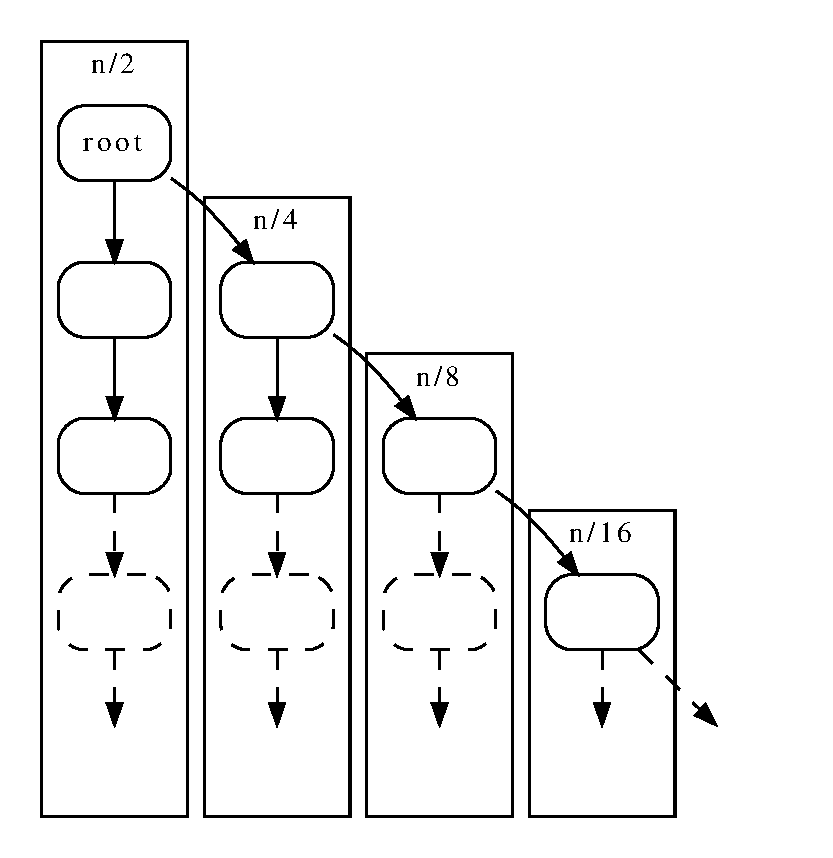
\includegraphics[scale=0.7]{bamboos.dot.eps}
\centering
\caption{Числа над каждым из бамбуков --- его длина, пунктирные стрелки --- продолжение дерева}
\end{figure}

Оба ребенка есть только в корнях бамбуков. В $i$-том корне у левого ребенка высота $\cfrac{n}{2^i}$, у правого $\cfrac{n}{2^{i+1}}$. Таким образом, рассматриваемое дерево подходит в условие. Высота этого дерева $\geq$ высота первого бамбука $=\cfrac{n}{2}\not=O(\log n)$. Итого, найдено дерево, подходящее в условие, в котором высота $\not=O(\log n) \Rightarrow$ ответ --- нет.

\end{document}